\documentclass[hyperref={pdfpagelabels=false},12pt]{beamer}
\usepackage[utf8]{inputenc}
%\usepackage{multirow}
%\usepackage{wasysym}
%\usepackage{upquote}
\usepackage{listings}
\usepackage{gensymb}
\usepackage{array}
\usepackage{times}
\usepackage{xcolor}
\usepackage{default}
\usepackage{ulem}

%\usetheme{Pittsburgh}

\xdefinecolor{darkgreen}{rgb}{0.11,0.64,0.22}
\title[Pitt Access]{{\large Pitt-ACCESS\\ A Comprehensive and Critical Evaluation System for Software}}
\author[Pitt-Access]{{Ketan and Barry}}
\date{}

\beamertemplatenavigationsymbolsempty


\begin{document}
\begin{frame}[plain]
\titlepage
\end{frame}

%Introduction
\begin{frame}
\frametitle{Motivation: Why do we want to do this?}
\begin{itemize}
\itemsep1em
\item 
Frustration with science software: architectures, installation, runtime, maintenance, dependencies, platforms, libraries, tools, compilers
\item 
Lack of an independent, neutral and critical evaluation platform: quantitative and qualitative
\item 
Benefit from a strong scientific computing infrastructure: applications, tools, techniques, technology
\end{itemize}
\end{frame}

\begin{frame}
\frametitle{Some Concrete Examples}
\begin{itemize}
\itemsep1em
\item Buildtime: GridPack Power Grid Simulation app from LLNL does not build on IBM BG/Q because it makes a fancy Boost library call. The call was not tested for BG/Q!
\item Runtime: Icenine image reconstruction app from CMU segfaults with \texttt{-O2} compiler flag of GCC
\item Install troubles: No makerule to statically build DISCUS: a diffusion scattering simulator
\item Qualitative: Rosetta suite uses the SCONES build system: extremely tedious to customize builds.
\end{itemize}
\end{frame}

\begin{frame}
\frametitle{Details: What Pitt-ACCESS is all about?}
\begin{itemize}
\itemsep1em
\item 
Mission: Build a community driven platform to \textbf{critically} evaluate science software.
\item 
Answers to questions such as:
\begin{itemize}
\item 
I need an MD software for the Nvidia/CUDA platform, which one to select?
\item 
Does this Combustion Engine Simulator deploy over the new Intel architecture?
\item
How many file corruptions per year over a FreeNAS/ZFS based storage system?
\item 
Given 32G memory/node, how well does \textit{VASP} scale for 750 ion problem space?
\end{itemize}
\end{itemize}

\end{frame}

\begin{frame}
\frametitle{Architecture: What are the key components?}
\begin{itemize}
\item 
Layered architecture: User Interface (web portal), Test Framework, Evaluation Framework, Database, Storage
%\item
%User accounts management system: community contributes, reviews and rates
%\item
%Catalog: tag and locate
%\item
%Structured database for contents
\end{itemize}
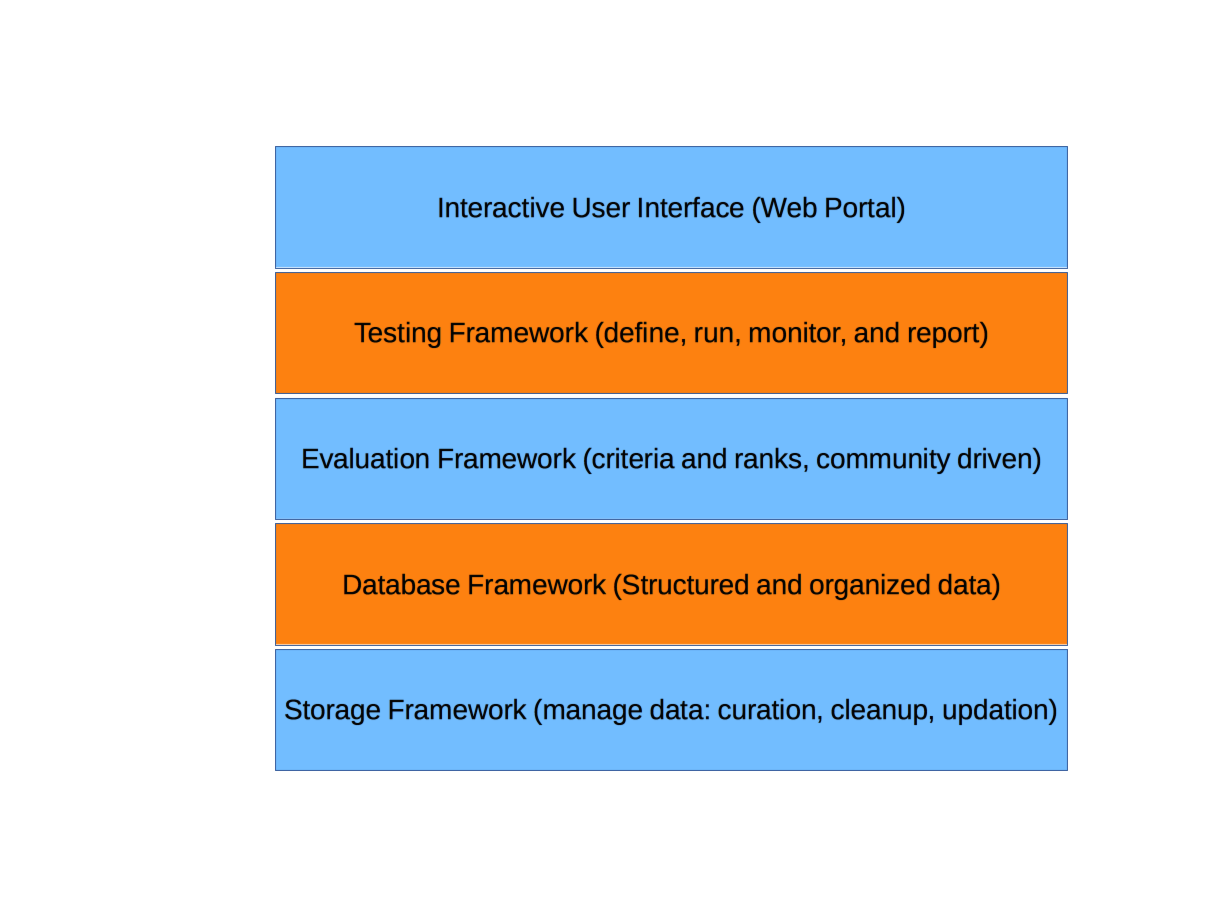
\includegraphics[width=9.6cm]{Architecture}
\end{frame}

\begin{frame}
\frametitle{Execution: Automated Software Evaluation Workflow}
\begin{center}
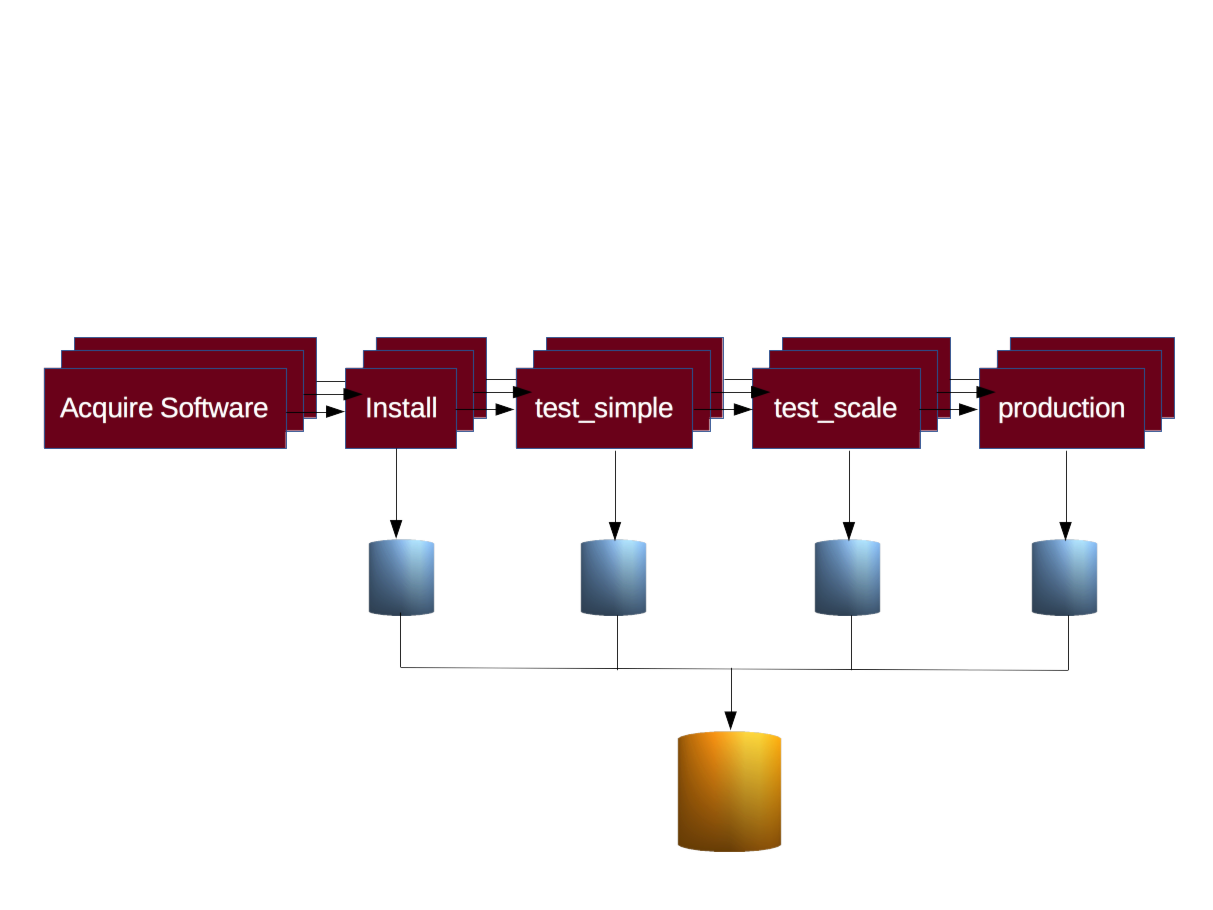
\includegraphics[width=11cm]{workflow}
\end{center}
\end{frame}

\begin{frame}
\frametitle{Challenges: Potential Roadblocks}
\begin{itemize}
\itemsep1em
\item
Technological: Be on the same page with current technology and what users are using
\item 
Strategic: potentially making important people upset (OTOH they are happy because their app gets more traction!)
\item
Legal: licensing issues, what to publish and what to withhold (start with ``local" software)
\item
 Sustainability: How do we sustain the effort?
\end{itemize}
\end{frame}

\begin{frame}
\frametitle{Benefits: What are the benefits?}
\begin{itemize}
\itemsep1em
\item Strengthen SaM's (and Pitt's) software infrastructure
\item
Save time and money for SaM and users
\item
Strong community outreach elements: keep in touch with leaders/PIs 
\item
Deeper understanding of science software leads to better collaboration
\item
Discover new bugs and improve quality at code level
\end{itemize}
\end{frame}

\begin{frame}
\frametitle{Example results(1): comparative view of apps}
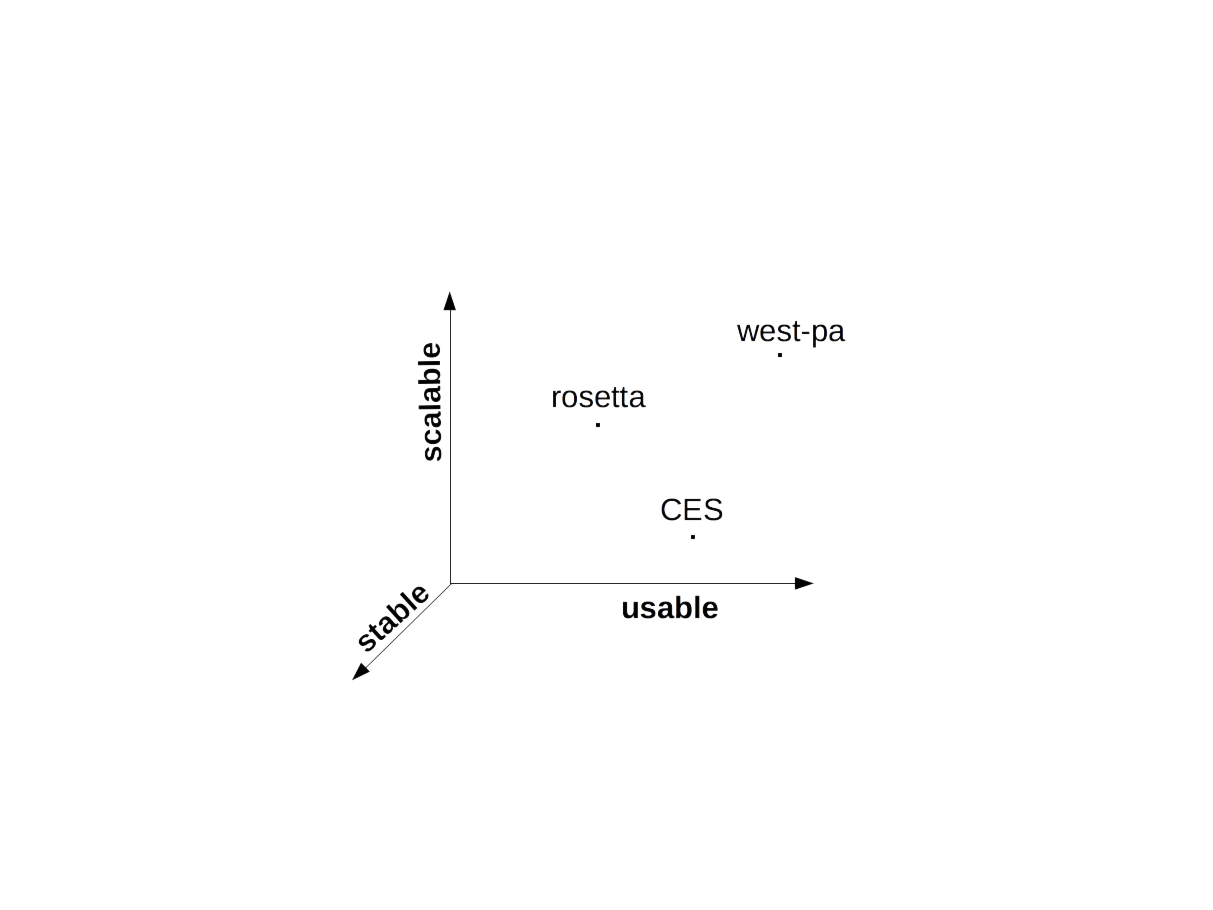
\includegraphics[width=9cm]{example1}
\end{frame}

\begin{frame}
\frametitle{(2): app vs compiler over a \textit{Dell cluster}}
\begin{table}
\begin{center}
% use packages: array
\begin{tabular}{|c|c|c|c|c|c|}
\hline
\textit{comp/app} & \textbf{ipopt} & \textbf{VASP} & \textbf{rosetta} & \textbf{dock} & \textbf{icenine} \\
\hline
\textbf{Intel Suite} & \checkmark & \checkmark & x & \checkmark & \checkmark \\
\hline
\textbf{GCC} & x & \checkmark & x & x & \checkmark \\
\hline
\textbf{PGI} & x & \checkmark & \checkmark & \checkmark & x \\
\hline
\textbf{clang} & \checkmark & x & x & \checkmark & x \\
\hline
\end{tabular}
\end{center}
\end{table}
\end{frame}

\begin{frame}
\frametitle{Is it well-aligned to SaM's mission: Why yes ... yes it is!}
\begin{itemize}
\itemsep1em
\item 
Promote multi-disciplinary research
\item
Enrich knowledge base
\item
Funding opportunities: Build partnerships with PIs/Groups
\item
A long term activity and effort!
\end{itemize}
\end{frame}

\begin{frame}
\frametitle{Plan: Timeline of activities }
\begin{itemize}
\itemsep1em
\item Quarter 1-2: design, test, feedback--Perform the acquire, install, test, run, scale cycle
\item Identify tools to build the platform: django/flask?, sqlite3?, json?, ...
\item Quarter 3-4: Narrow down scope, short term goals, select target software, first webpage goes live
\item Add more software, diversify science domain
\item Identify and register patterns, eg. dominant IO patterns adapted by apps
\end{itemize}
\end{frame}

\begin{frame}
\frametitle{Summary: IMDb of science software!}
\begin{itemize}
\itemsep1em
\item Valuable at all scales, many fringe benefits
\item Broader, deeper community engagement and outreach
\item Contribution to multi-disciplinary software infrastructure
\item Future: a multi-disciplinary application development center
\end{itemize}
\end{frame}

\begin{frame}
\frametitle{\\ \centering Thank you for your attention! \\ We are looking for comments and feedback!}
\end{frame}

\end{document}

